\documentclass[tikz,border=3mm]{standalone}
\usetikzlibrary{positioning, shapes.geometric, arrows.meta, calc}

\begin{document}
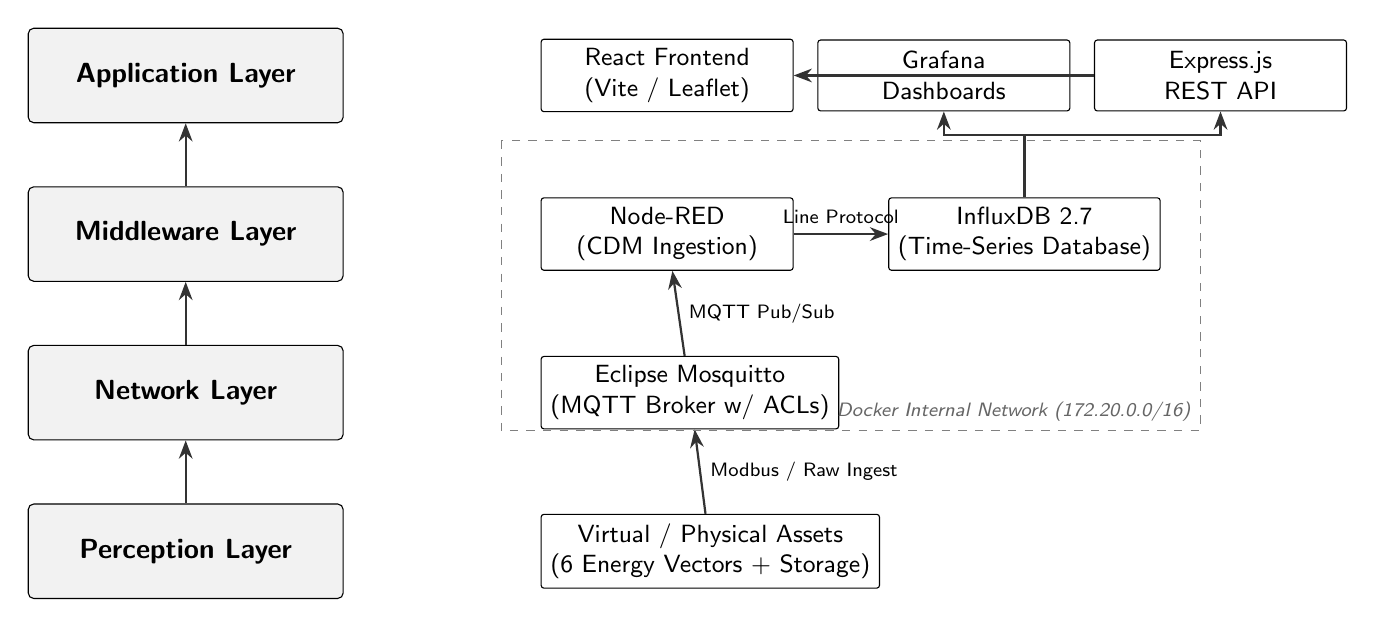
\begin{tikzpicture}[
    layer/.style={draw, fill=black!5, minimum width=4cm, minimum height=1.2cm, align=center, font=\bfseries\sffamily, rounded corners=2pt},
    comp/.style={draw, fill=white, minimum width=3.2cm, minimum height=0.9cm, align=center, font=\sffamily\small, rounded corners=1pt},
    arrow/.style={-Stealth, thick, draw=black!80},
    title/.style={font=\bfseries\sffamily\large}
]

    % Draw Layers (Left Column)
    \node[layer] (L4) {Application Layer};
    \node[layer, below=0.8cm of L4] (L3) {Middleware Layer};
    \node[layer, below=0.8cm of L3] (L2) {Network Layer};
    \node[layer, below=0.8cm of L2] (L1) {Perception Layer};

    % Draw Components (Right Column)
    \node[comp, right=2.5cm of L4] (C4a) {React Frontend\\(Vite / Leaflet)};
    \node[comp, right=0.3cm of C4a] (C4b) {Grafana\\Dashboards};
    \node[comp, right=0.3cm of C4b] (C4c) {Express.js\\REST API};
    
    \node[comp, right=2.5cm of L3] (C3a) {Node-RED\\(CDM Ingestion)};
    \node[comp, right=1.2cm of C3a] (C3b) {InfluxDB 2.7\\(Time-Series Database)};
    
    \node[comp, right=2.5cm of L2] (C2) {Eclipse Mosquitto\\(MQTT Broker w/ ACLs)};
    
    \node[comp, right=2.5cm of L1] (C1) {Virtual / Physical Assets\\(6 Energy Vectors + Storage)};

    % Layer Connectors
    \draw[arrow] (L1) -- (L2);
    \draw[arrow] (L2) -- (L3);
    \draw[arrow] (L3) -- (L4);

    % Component Connections
    \draw[arrow] (C1) -- node[right, font=\sffamily\scriptsize] {Modbus / Raw Ingest} (C2);
    \draw[arrow] (C2) -- node[right, font=\sffamily\scriptsize] {MQTT Pub/Sub} (C3a);
    \draw[arrow] (C3a) -- node[above, font=\sffamily\scriptsize] {Line Protocol} (C3b);
    
    % Middleware to Apps
    \draw[arrow] (C3b) |- ($(C4b.south) + (0,-0.3)$) -- (C4b.south);
    \draw[arrow] (C3b) |- ($(C4c.south) + (0,-0.3)$) -- (C4c.south);
    \draw[arrow] (C4c) -- (C4a);

    % Outer boundary representing Docker Internal Network
    \draw[dashed, black!50] ($(C2.west) + (-0.5, 3.2)$) rectangle ($(C3b.east) + (0.5, -2.5)$);
    \node[font=\sffamily\scriptsize\itshape, text=black!60, anchor=south east] at ($(C3b.east) + (0.5, -2.5)$) {Docker Internal Network (172.20.0.0/16)};

\end{tikzpicture}
\end{document}
